\pagestyle{empty}
\cleardoublepage
\pagestyle{fancy}

\chapter{Modelagem Dinâmica e Controlador} \label{Cap:Modelagem:Dinamica}

 Nesse capítulo, abordaremos a modelagem dinâmica do rotor que sofre influências das forças do estator externo e dos polos do estator interno. Um modelo linearizado no ponto de operação é apresentado para o projeto do controlador.
 
\section{Modelagem}

A dinâmica do rotor é influenciada basicamente pela sua velocidade de rotação ($\dot{\theta}$), sua inércia ($I$), sua massa ($m$) e posição relativa do rotor ($d_x,d_y,d_z$), compondo a energia cinética ($T$) do sistema. A parcela da energia potência ($V$) se dá pela sua translação axial ($d_z$), pela gravidade ($g$) e pela rigidez passiva do mancal ($K_z$) calculada na \todo{sem referencia} Sec. \ref{}. A Fig. \ref{fig:modelo:forcas} ilustra as forças atuantes no rotor, sendo:

 \begin{itemize}
 	\item $F_p$ : Força devido ao ímã permanente
 	\item $F_b$ : Força devido a bobina
 	\item $\tau$ : Torque de rotação devido ao motor
 	\item $\theta$ : O angulo do rotor
 	\item $x,y,z$ : Deslocamento no plano cartesiano 
 \end{itemize}

 \begin{figure}[th]
 	\centering
 	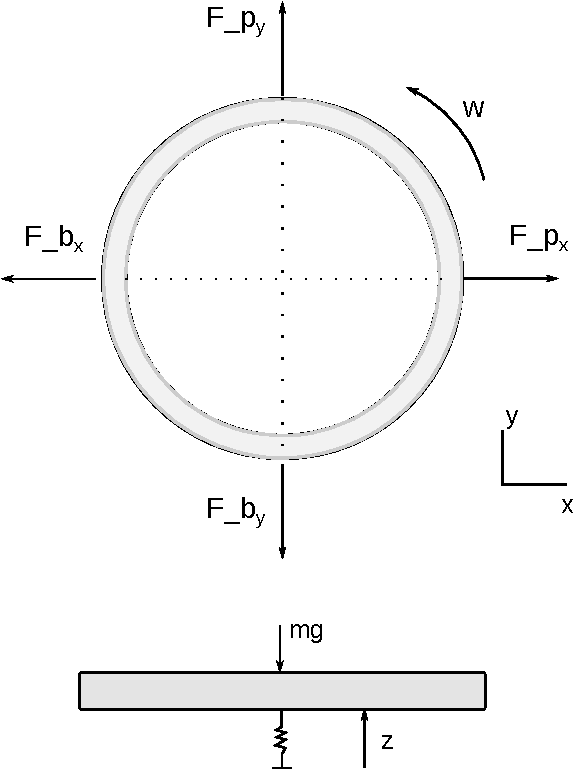
\includegraphics[width=0.7\linewidth]{../Figs/Modelagem/forcas}
 	\caption{Forças atuantes rotor}
 	\label{fig:modelo:forcas}
 \end{figure}
 
 \begin{align}
 	T_{\theta, x, y, z} &= \frac{1}{2} I_z \, \dot{\theta}^2 + \frac{1}{2} \, m \, \left( \dot{x}^2 + \dot{y}^2 + \dot{z}^2 \right) \notag \\
 	V_z &= m \, g \, z + \frac{1}{2} \, K_z \, z^2
 \end{align}	
 	
 Duas forças distintas agem no rotor: a primeira, não conservativa ($Q^{nc}$) é causada pela força de atração ($F_b$) nos atuadores, é dependente da posição do rotor e da corrente aplicada ($i$); a segunda, conservativa ($Q^{c}$) é dependente somente da posição do rotor e é causada pela força de atração dos ímãs, podendo ser traduzida para uma rigidez ($K_p$). Ambas as forças $F_b$ e $K_p$ são levantadas via o modelo de elementos finitos. 
	 	
 \begin{align}
 	Q_y^{nc} &= F_{by}(x,i)  \\
 	Q_x^{nc} &= F_{bx}(y,i)  \\
 	Q^{c}_x  &= K_p \, x \\
 	Q^{c}_y  &= K_p \, y 
 \end{align}
  
  Com a resolução da lagrangiana (Eq. \ref{eq:dinamica:lagrangiana}) obtivemos as equações da dinâmica do sistema (Eq. \ref{eq:dinamica:modelo}):
  
   \begin{align}
   		L = T - V \notag \\
   		\frac{\partial}{\partial t} \left[ \frac{\partial L}{\partial \dot{r}} \right] -  \frac{\partial L}{\partial r} = Q^{nc} + Q^{c}
   		\label{eq:dinamica:lagrangiana}
   \end{align}
  
 	\begin{align}
 	I \ddot{\theta} &= 0 \\
 	m \ddot{x}		&= K_p \, x  - F_{bx}(x,i) \\
 	m \ddot{y}		&= K_p \, y  - F_{by}(y,i) \label{eq:dinamica:rotor:radial}\\	
 	m \ddot{z}  	&= K_z \, z + m g 
 	\label{eq:dinamica:modelo}
 	\end{align}	
 
 Exceto pela dependência das posições nas forças, verificamos, pelas equações, o desacoplamento entre os diferentes graus de liberdade. 

\subsection{Rigidez Passiva: $K_p$}

A força exercida no rotor devido aos ímãs permanentes do estator externo pode ser aproximada por uma equação linear, como visto em \ref{subsection:forca:x}. Assumisse que a força de atração no roto para pequenos deslocamento dependa somente da posição no eixo, podendo ser representada pela decomposição:\todo{última frase confusa, tire esse assumisse}

\begin{align}
	F_p(x) &= K_p \, x \\
	F_p(y) &= K_p \, y 
\end{align}

Onde $K_p$ é a constante de proporção entre a força e a posição e x e y são os deslocamento em torno do ponto de equilíbrio do rotor com relação ao estator externo. Obtivemos, via a simulação em elementos finitos, uma relação força por deslocamento para ambos os eixos (devido a simetria do mancal). 

\begin{equation}
 K_p(d) = 625 N/mm 
\end{equation}

\subsection{Rigidez Ativa : $F_b$}

A força de atração do rotor devido ao campo magnético gerado pelas bobinas é não linear com a posição do rotor (comprimento do entreferro) e depende da corrente de excitação aplicada às bobinas.  

As tensões nas bobinas são distribuídas conforme Fig. \ref{fig:blocos:tensao:bobinas:x:y} (a), onde existe sobreposição de bobinas para atuação em diferentes eixos (X e Y). É aplicada nas bobinas que possuem sobreposição a metade da tensão, limitando assim o valor da tensão total nas bobinas para o valor máximo (I/2 + I/2 = $I_max$). A Fig. \ref{fig:blocos:tensao:bobinas:x:y} ilustra a configuração proposta. Verificamos que a tensão é aplicada em metade para as bobinas com sobreposição (a,g,e,c) e com ganho unitário nas bobinas principais (h,f,c,b). 

\begin{figure}[th]
\centering
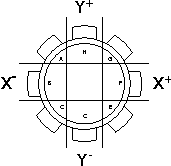
\includegraphics[width=0.7\linewidth]{./Figs/Modelagem/ativo-atuadores-conexao}
\caption{Distribuição das tensões nas bobinas}
\label{fig:blocos:tensao:bobinas:x:y}
\end{figure}

A força aplicada no rotor fi levantada via resultados da modelagem em elementos
finitos, um polinômio de segundo grau com confidência de 95\% foi encontrado
(Eq. \ref{eq:fb:segundo:grau}) via curva da Fig.
\ref{ativo_otimizado_fem_I_dx_map}, os coeficientes estão descritos na Tab. \ref{tab:dinamico:ajuste:kb}.

\begin{align}
     fit_Kb(dx,I) &= p00 + p10*dx + p01*I + p20*dx^2 +\\
     & p11*dx*I + p02*I^2 + p30*dx^3 + p21*dx^2*I +\\
     & p12*dx*I^2 + p03*I^3
     \label{eq:fb:segundo:grau}
\end{align}

\begin{table}[ht!]
\centering
\begin{tabular}{c l}
	   p00 & -3.25\\
	   p10 & -5.17\\
	   p01 &  24.13\\
	   p20 &   98.13\\
	   p11 & -90.04\\
	   p02 &  22.83\\
	   p30 &   -146\\
	   p21 &  22.29\\
	   p12 &  9.44	\\
	   p03 & -3.79
\end{tabular} 
\caption{Coeficientes do ajuste à curva de ganho Kb}
\label{tab:dinamico:ajuste:kb}
\end{table}

\subsection{Dinâmica do Atuador}

Devido as bobinas dos polos do estator interno, uma dinâmica do atuador ($G_a(s)$) atrelada a indutância deve ser considerada. A bobina é modelada como um circuito RL, com a dinâmica descrita na Eq. \eqref{eq:dinamica:bobina}.

\begin{align}
	I(s) &= \frac{V(s)}{R + L \, s} 
	\label{eq:dinamica:bobina}
\end{align}

Os valores das indutâncias são calculados como demonstrada na SubSec. \ref{subsec:at:indutancia}. Os valores nominais no ponto de operação de cada bobina é de aproximadamente $76 \, \mu H$ e a sua resistência elétrica de 6.3 $\Omega$ causando uma frequência de corte de $13$ kHz. 

As tabelas \ref{tab:dinamica:indutancia} e \ref{tab:dinamica:indutancia:mutua} demonstram a evolução da indutância principal (L) e da mutua (M) quando uma corrente de 4 Ampères é aplicada no polo principal. 

\begin{table}[ht!]
	\centering
	\begin{tabular}{c c}
        L [uH]  & $d_x$ [mm] \\
        \hline \hline               
        78.013 & 0.00 \\
        77.450 & 0.05 \\
        76.890 & 0.10 \\
        76.333 & 0.15 \\
        75.710 & 0.20 \\
        75.048 & 0.25 \\
        74.381 & 0.30       
	\end{tabular} 
	\caption{Indutância calculada para um único polo em diversos pontos de operação via elementos finitos. Corrente aplicada de 4 Ampères no polo principal}
	\label{tab:dinamica:indutancia} 
\end{table} 

\begin{table}[ht!]
	\centering
	\begin{tabular}{c c}
        M [uH]  & $d_x$ [mm] \\
        \hline \hline               
         18.693 & 0.00 \\
         18.327 & 0.05 \\
         17.979 & 0.10 \\
         17.638 & 0.15 \\
         17.303 & 0.20 \\
         16.988 & 0.25 \\
         16.662 & 0.30       
	\end{tabular} 
	\caption{Indutâncias mutua calculada para um único polo em diversos pontos de operação via elementos finitos. Corrente aplicada de 4 Ampères no polo principal}
	\label{tab:dinamica:indutancia:mutua} 
\end{table} 

Uma aproximação linear das indutâncias foi calculada (Eq. \ref{eq:indutancias:aprox}) para a utilização na modelagem não linear. Essas equações demonstram a sensibilidade que um sensor de indutância teria que ter, em uma futura implementação, para a leitura da posição relativa do rotor via a indutância dos polos.

\begin{align}
	L(x) &= -1.206 \,10^{-5} x + 2.807 \, 10^{-5} \\
	M(x) &= -6.756 \,10^{-6} x + 1.867 \, 10^{-6} 
	\label{eq:indutancias:aprox}
\end{align} 

\subsection{Batente}

O batente atua como uma saturação na posição do rotor (x,y, z), atrelou-se uma dinâmica ao batente para analisar as influências de choques mecânicos do rotor, possibilitando a análise de fadigas e a especificação de componentes de fixação (parafusos). Utilizou-se no  modelo o módulo de elasticidade de Young, onde a penetração ($\Delta l $) no material pode ser calculada por:

\begin{equation}
	\Delta l =  \frac{F l_o}{E \, A}
\end{equation}

Sendo : \textbf{E }a constante de Yomg para o material; \textbf{A} área de contato; \textbf{$l_o$ } o comprimento inicial do material e \textbf{F} a força resultante do impacto. 


\subsection{Modelo Linear}

O modelo linear ($G_{ma}$) de malha aberta para um dos eixos de movimentação no plano x,y (radial) foi levantado em torno do equilíbrio do rotor, considerou-se as dinâmicas do rotor ($G_r$) e do atuador ($G_a$) deduzidas das equações  \eqref{eq:dinamica:rotor:radial} e \eqref{eq:dinamica:bobina}.

\begin{align}
	G_r &= \frac{1}{s^2 \, m - K_p} \\
	G_a &= \frac{K_b}{s\, L + R}
\end{align}

O modelo encontrado foi utilizado para o projeto do controlador ($C(s)$), esse otimizado para operar em torno do ponto de operação (rotor). A função transferência do modelo obtido é demonstrada na Eq. \eqref{eq:dinamica:tfunc:gen}, o sistema obtido possui três polos sendo \todo{não seria: "...três polos nenhum deles seno integrador puro"?}eles nenhum integrador puro (sistema tipo 0).  

\begin{align}
	G_{ma}(s) &= \frac{K_b}{(s^2 \, m - K_p) \, (s\, L + R)}	\label{eq:dinamica:tfunc:gen} \\
	&= \frac{58}{(s^2 \, 0.375 - 625) \, (s\, 7.8 \, 10^{-5} + 6.3)}
	 \label{eq:dinamica:tfunc}
\end{align}
 

Os três polos estão localizado em: $[-82E3 -41 +41]	$, onde a função de transferência é descrita na Eq. \eqref{eq:dinamica:tfunc}, os parâmetros utilizados foram encontrados nas \todo{precisa de referência?}secções anteriores. 

Verificou-se que o sistema é instável em malha aberta e um controlador deve ser projetado para estabilizá-lo. 

\subsection{Modelo Dinâmico Não Linear}

Um modelo dinâmico não linear foi projetado em ambiente Matlab Simulink para a validação do controlador, esse modelo, leva em consideração as modelagens eletromagnéticas realizadas para a otimização do mancal.

A Fig. \ref{fig:diagrama:blocos:modelo:linear} demonstra o diagrama de blocos proposto, sendo $C_s$ o controlador projetado. Nesse esquema, o controlador age diretamente nas bobinas aplicando a corrente necessária para estabilizar o rotor no ponto de operação. 

\begin{figure}[th!]
	\centering
	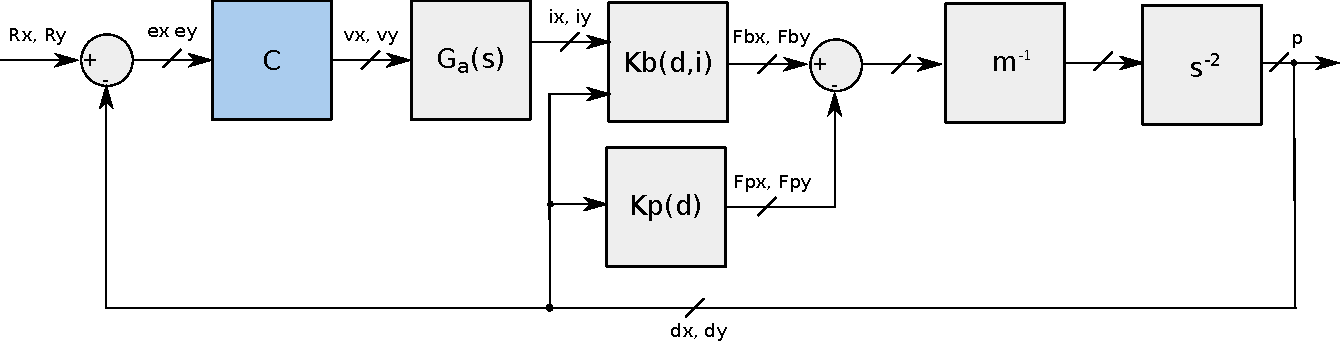
\includegraphics[width=1\linewidth]{../Figs/Modelagem/diagrama_blocos_modelo_linear}
	\caption{Diagrama de blocos do modelo linearizado para descolamentos em x e y}
	\label{fig:diagrama:blocos:modelo:linear}
\end{figure}

Duas saturações devem ser consideradas, a primeira, referente a tensão da bobina deve ser limitada ao seu valor máximo (30V) e a segunda saturação que é causada pelo batente do rotor e que limita sua excursão máxima.

\section{Projeto do Controlador}

Um controlador foi projetado a fim de demonstrar a controlabilidade do sistema proposto dentro das especificações impostas ao mancal. O projeto do controlador foi feito via modelo linear e validado utilizando o modelo não linear. 

O controlador age diretamente sob a posição do rotor no plano x,y através de duas forças ortogonais: $F_{bx}$ e $F_{by}$. A corrente necessária para gerar essas forças foi calculada via um estimador de corrente que traduziu a força imposta pelo controlador na corrente necessária levando em consideração a posição do rotor.

%Um estimador de forças é proposto a fim de minimizar as variações do ganho do atuador, o controlador age não diretamente sobre a corrente mas sim sobre a força necessária para estabilizar o rotor. O estimador é responsável por traduzir a força imposta pelo controlador em uma corrente.

\subsection{Estimador}
	
A fim de superar as não linearidades no ganho do atuador ($Kb(d,i)$), um controle de força foi projetado no lugar do de corrente. A força calculada pelo controle ($F_b$) foi aplicada em um estimador que calculou a corrente necessária a ser aplicada na bobina com base na posição do rotor. A Fig. \ref{fig:diagrama_controlador_estimador} demonstra o estimador de corrente proposto. O mesmo é dependente da área do polo ($S_n$), do comprimento do entreferro ($l_g$) e do número de \todo{chama espirar mesmo?}espirar ($n_n$). O equacionamento (Eq. \eqref{eq:estimator:i}) foi obtido através de um modelo simplificado da equação de força magnética considerando apenas um entreferro e um componente ferromagnético.

%\begin{align}
%F_b &= \frac{B_g^2 \m S_n}{2\, \mu_0} \\
%H_g \mu_0 &= B_g 
%\end{align}
	
\begin{equation}
I = \sqrt{\frac{2 \, F_b \, \mu_0}{S_n}} \, \frac{l_g \mu_0}{n_n}
\label{eq:estimator:i}
\end{equation}
	
Um exemplo da variação do ganho do atuador ($K_b$) pode ser ilustrado em dois cenários distintos, o primeiro, quando o rotor está em seu ponto de operação, sua força de atração gerada pela aplicação de uma corrente de 4A é 209 Newton, segundo quando o rotor encontra-se em seu deslocamento máximo ($d_x = 0.3 mm$) e a força resultante é de apenas 120N.

\begin{figure}[ht!]
	\centering
	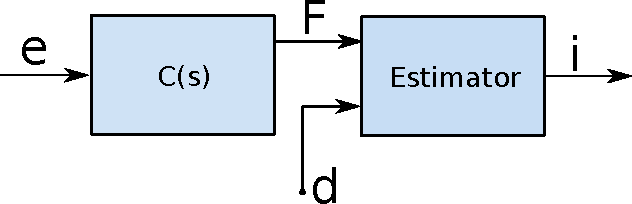
\includegraphics[width=0.5\linewidth]{Figs/Modelagem/controlador_estimador}
	\caption{Diagrama de blocos do controlador e do estimador}
	\label{fig:diagrama_controlador_estimador}
\end{figure}

\subsection{Controlador}

O controlador proposto para o mancal magnético é um controle do tipo Proporcional (P), Integral (I) e Derivativo (D), com a estrutura da Eq. \eqref{eq:controle:pid}, um filtro (N) foi aplicado ao fator derivativo a fim de evitar que ruídos provenientes do sensor fossem amplificados pelo controlador.

\begin{align}
	C(s) = P \, \left( 1 + \frac{I}{s} + \frac{N \, D}{ 1 + \frac{N}{s}} \right)
	\label{eq:controle:pid}
\end{align}

O controlador foi projetado considerando o ganho unitário da bobina ($K_b = 1$), isso foi necessário para gerar um controlador que possuísse a força como esforço de controle e não a corrente. A saída do controlador foi aplicada ao estimador que traduziu, por sua vez, a força em tensão necessária à bobina. 

Devido a instabilidade do sistema em malha aberta e as variações do ganho do atuador de forma não linear com a movimentação do rotor, optou-se por projetar um controlador privilegiando a robustez ao invés da agressividade.

O controlador obtido via especificação possui os ganhos da Tab. \ref{tab:controle:pid}:

\begin{table}[ht!]
\centering
	\begin{tabular}{c c c c}
	 kp  &  ki & kd &  N  \\
	 \hline \hline
		1926	 &	5.89	& 0.017	&1616
	\end{tabular} 
	\caption{Ganhos do controlador PID}
	\label{tab:controle:pid}
\end{table}


	\begin{figure}[!ht]
	\centering
		\subfloat[t][Diagrama de bode]{
			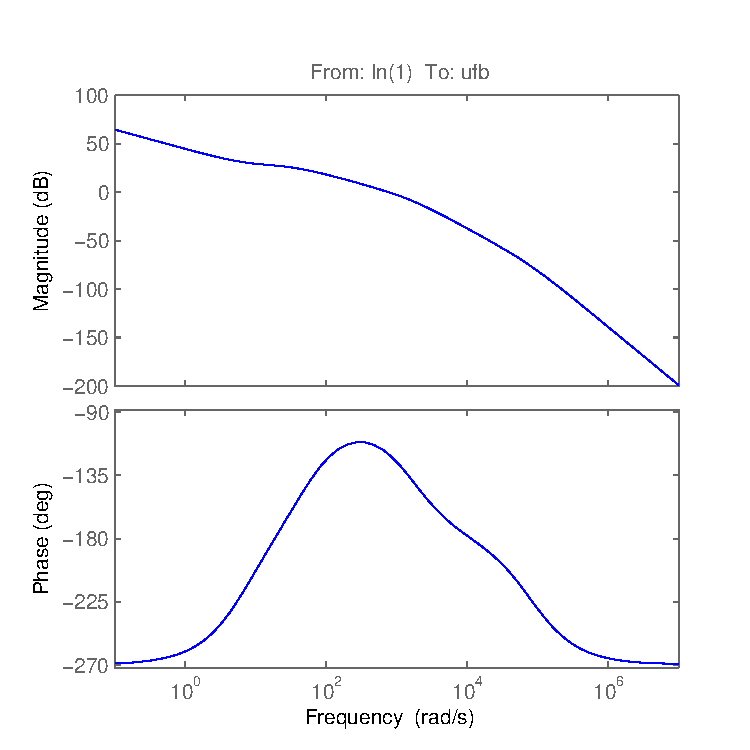
\includegraphics[width=0.5\linewidth]{Figs/controle/bode_pid_g}
		}
		%
		\subfloat[b][Lugar das raizes]{
			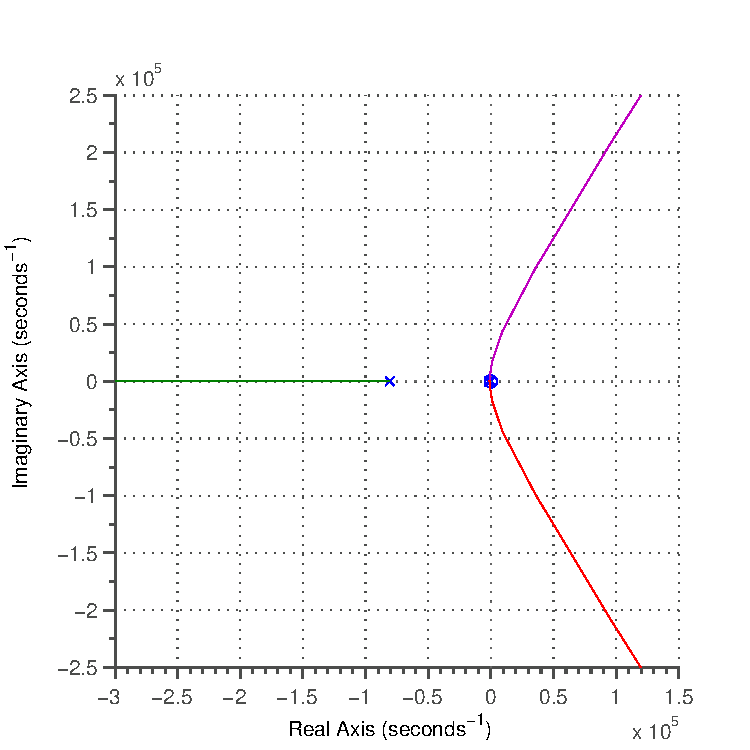
\includegraphics[width=0.5\linewidth]{Figs/controle/rlocus_pid_g}
		}	\\
		\subfloat[c][Resposta ao degrau do sistema em malha fechada com o controlador PID, sistema linearizado]{
		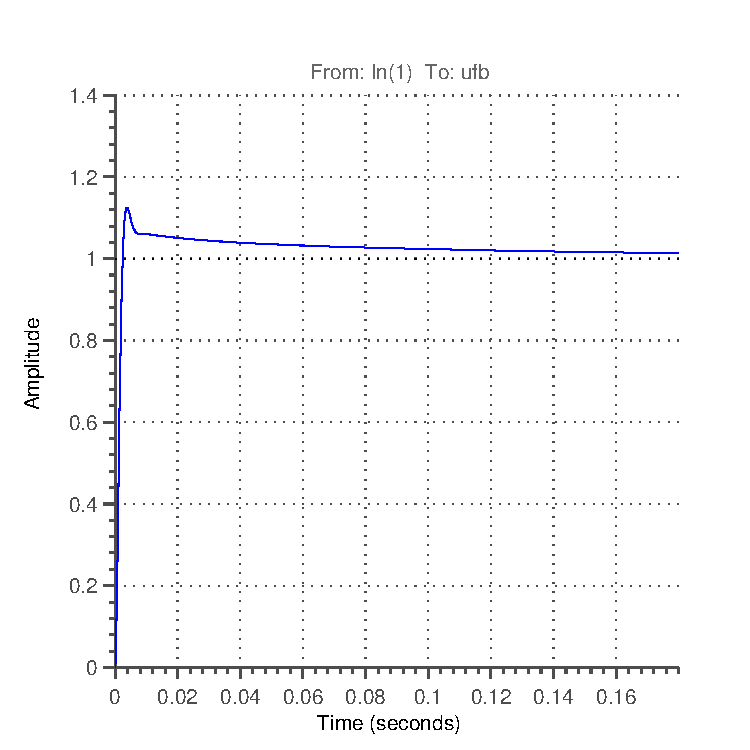
\includegraphics[width=0.7\linewidth]{Figs/controle/step_pid_g}
		}
		\caption{Análise do sistema controlado, diagrama de bode e lugar das raízes}
		\label{Fig:controle:analise}
	\end{figure}

O controle obtido impôs uma estabilidade no mancal com 60 graus de margem de fase e 27.8 dB margem de ganho. O tempo de acomodação foi de 123 ms com sobressinal de 12 \%. A resposta ao degrau está demonstrada na Fig. \ref{Fig:controle:analise}

\begin{figure}[ht!]
\centering

\label{fig:controle:degrau}
\end{figure}

A simulação do controle PID com o estimador no sistema com ganhos variáveis está demonstrada na Fig. \ref{fig:pid_nlinear_degrau}, notamos que a resposta do sistema sofreu alterações quando comparada com a do modelo linear. Essas alterações são causadas basicamente pela variação da indutância com o decorrer da posição do rotor e, principalmente, pela variação do ganho do atuador.

\begin{figure}
\centering
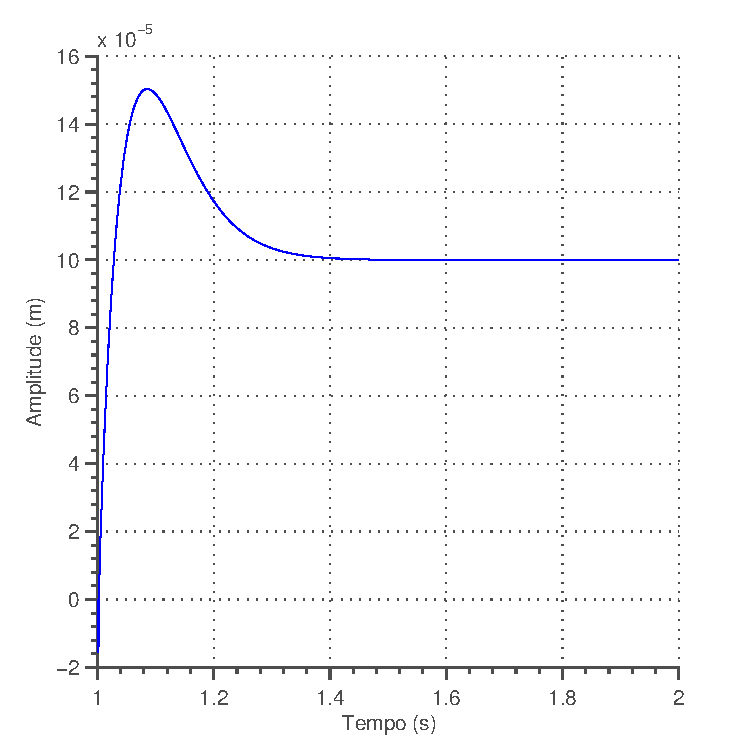
\includegraphics[width=0.7\linewidth]{Figs/controle/pid_nlinear_degrau}
\caption{Resposta ao degrau do sistema em malha fechada com o controlador PID, sistema não linearizado}
\label{fig:pid_nlinear_degrau}
\end{figure}

